\documentclass[tikz]{standalone}


\usepackage{graphicx}
\usepackage{pxfonts}
\newcommand{\figf}{\sffamily\bfseries}

\begin{document}
\sffamily

\begin{tikzpicture}[anchor = north west]

	\clip (0,0) rectangle +(18,-9);

	\begin{scope}
		\node[scale=0.8] at (0,0) {\includegraphics[page=2]{../img/model-setup.pdf}};
		\node at (0,0) {\figf A};
	\end{scope}


	\begin{scope}[yshift=-4.9cm]
		\node[scale=0.9] at (0,-0.1) {\includegraphics{../plots/panelB.pdf}};
		\node at (0,0) {\figf B};
	\end{scope}

	\begin{scope}[yshift=-4.9cm, xshift=6.5cm]
		\node[scale=0.9] at (0,-0.1) {\includegraphics{../plots/panelC.pdf}};
		\node at (0,0) {\figf C};
	\end{scope}
	
	\begin{scope}[xshift=11.5cm]
		\clip (0,0) rectangle +(6.5,-5);
		\node at (0.25,-0.25) {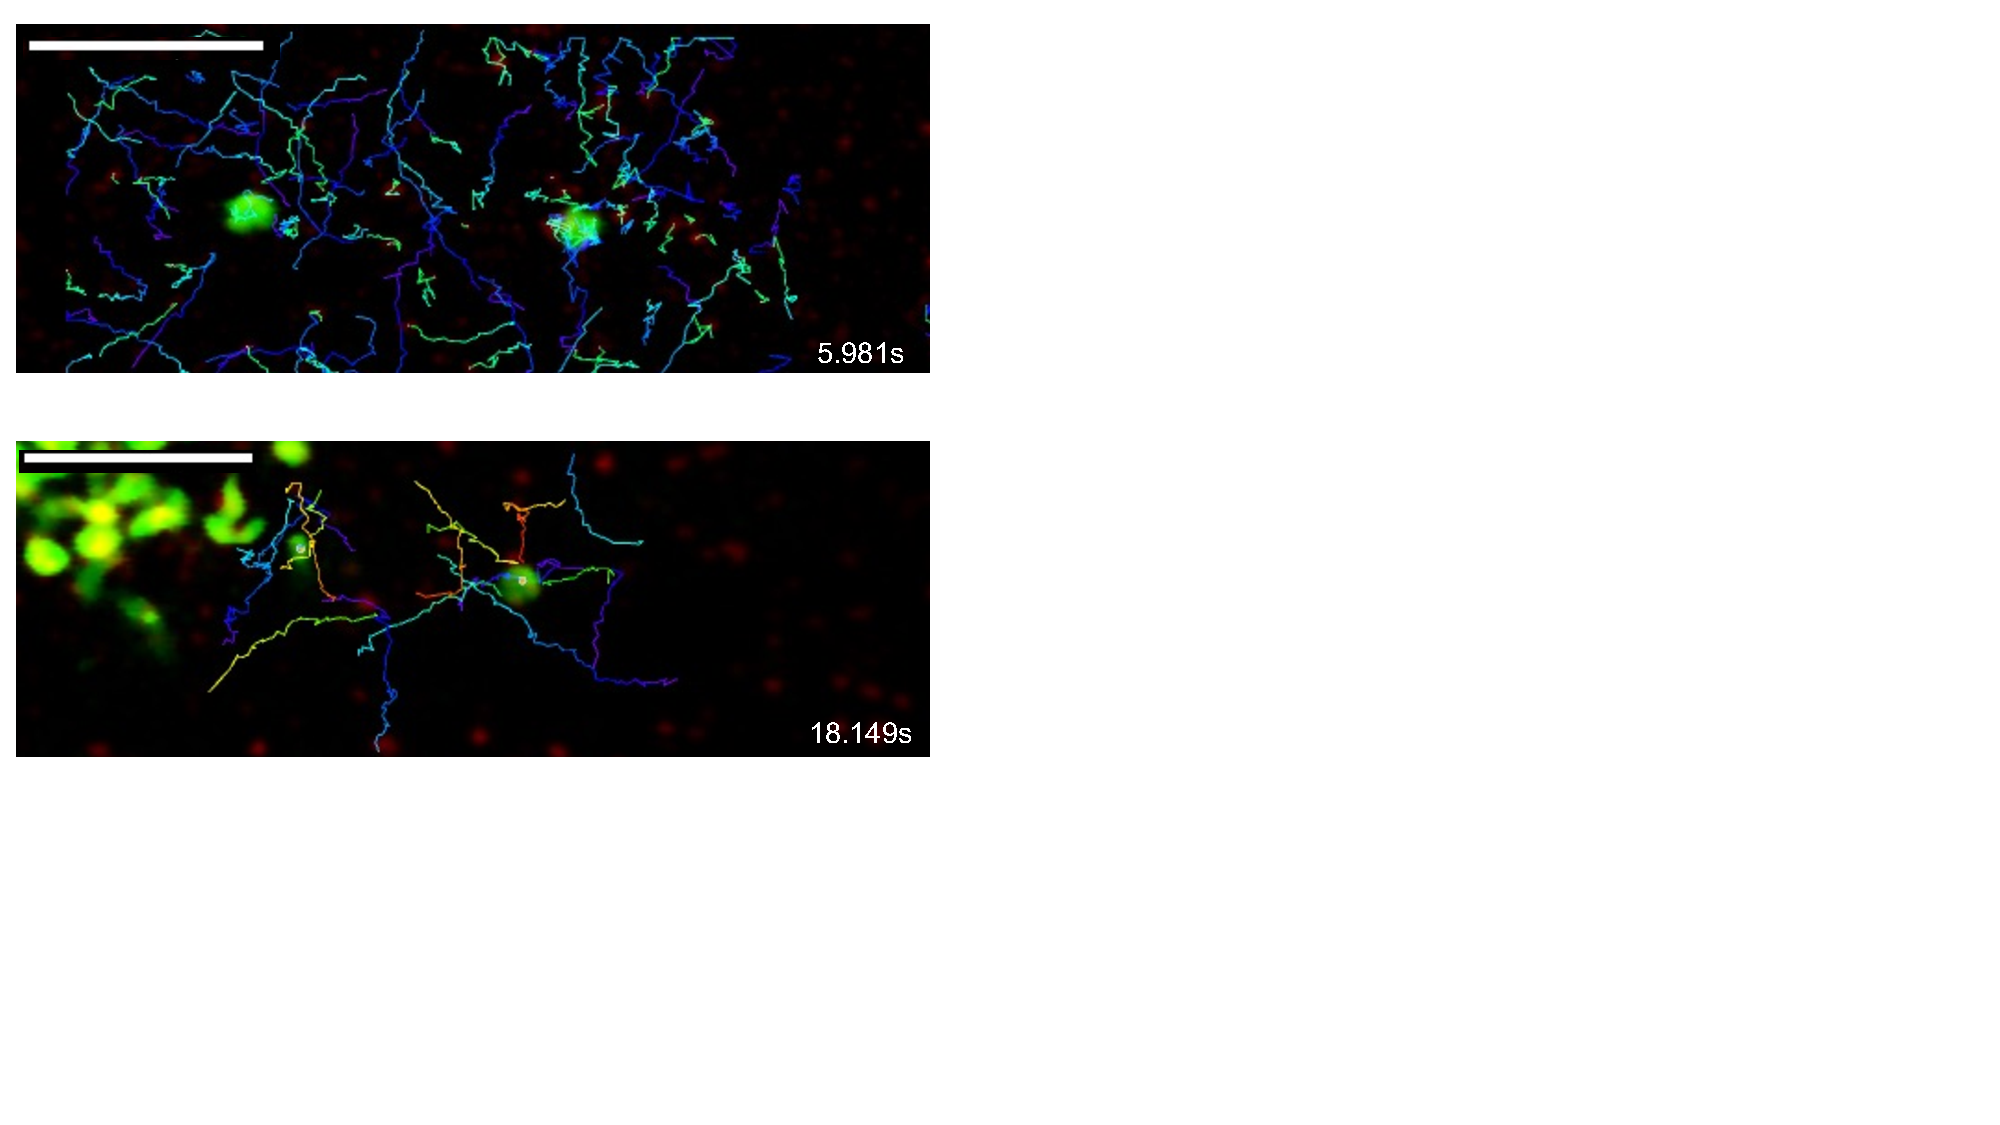
\includegraphics[width=11cm]{../img/fly-paper2.pdf}};
		\node at (0.35,-0.1) {\scriptsize in vitro};
		\node at (0.35,-2.4) {\scriptsize explant};
		\node at (0,0) {\figf D};
	\end{scope}

	\begin{scope}[xshift=13.5cm, yshift=-4.9cm]
		\node[scale=0.9] at (0,-0.28) {\includegraphics{../plots/panelE.pdf}};
		\node at (0,0) {\figf E};
	\end{scope}


\end{tikzpicture}

\end{document}